%%%%%%%%%%%%%%%%%%%%%%%%%%%%%%%%%%%%%%%%
% BCS LaTeX template
% Version: 1.2
%%%%%%%%%%%%%%%%%%%%%%%%%%%%%%%%%%%%%%%%
\documentclass[a4paper, DIV=12, abstracton]{scrreprt}
\setcounter{secnumdepth}{5}
\setcounter{tocdepth}{5}


%%%%%%%%%%%%%%%%%%%%%%%%%%%%%%%%%%%%%%%%
% author and thesis details (please adjust accordingly)
%%%%%%%%%%%%%%%%%%%%%%%%%%%%%%%%%%%%%%%%
\newcommand{\name}{Gizem Ekinci} % <-- your name here
\title{Bayesian Inference of Information Transfer in Graph-Based Continuous-Time Multi-Agent Systems} % <-- thesis title here
\newcommand{\documenttype}{Master-Thesis} % <-- select type: "Master-Thesis", "Bachelor-Thesis", "Projektseminar", "Proseminar"
\newcommand{\major}{Elektro- und Informationstechnik} % <-- your study program
\newcommand{\supervisor}{Dominik Linzner} % <-- your supervisor here
\newcommand{\submission}{07.07.2020} % <-- your submission date here
%%%%%%%%%%%%%%%%%%%%%%%%%%%%%%%%%%%%%%%%

%%% load document settings %%%
%%%%%%%%%%%%%%%%%%%%%%%%%%%%%%%%%%%%%%%%
% packages
%%%%%%%%%%%%%%%%%%%%%%%%%%%%%%%%%%%%%%%%

%%% math %%%
\usepackage{amsmath}
\usepackage{amssymb}
\usepackage{mathtools}
\usepackage{unicode-math}

%%% fonts %%%
\usepackage{lmodern}

%%% graphics %%%
\usepackage{tikz, wrapfig}
\graphicspath{{figures/}}
\usepackage{subcaption}
\usepackage{float}
\usepackage{graphicx}
\usetikzlibrary{positioning}
\usetikzlibrary{arrows}

%%% bibliography %%%
\bibliographystyle{plain}
\usepackage{etoolbox}
\AtBeginEnvironment{thebibliography}{\interlinepenalty=10000}

%%% misc %%%
\usepackage{blindtext}

%%% algorithms %%%
\usepackage{algorithmic}
\usepackage[ruled, lined, longend]{algorithm2e}

%%% referencing %%%
\usepackage[bookmarks, bookmarksdepth=chapter, hidelinks]{hyperref}
\usepackage[capitalise, noabbrev]{cleveref}
\newcommand{\crefrangeconjunction}{-}
\usepackage{xr}


%%%%%%%%%%%%%%%%%%%%%%%%%%%%%%%%%%%%%%%%
% document settings
%%%%%%%%%%%%%%%%%%%%%%%%%%%%%%%%%%%%%%%%

%%% title page %%%
\author{}
\date{}
\titlehead{
	\centering
	
\includegraphics[width=10cm]{tud_logo.pdf} \\
	\large\sffamily
	Fachbereich Elektrotechnik und Informationstechnik \\
	Bioinspired Communication Systems
	\vspace{10ex}
} 
\subtitle{
	\vspace{2ex}
	\documenttype\\
	\normalfont \sffamily 
	\major \\
	\vspace{4ex}
	Eingereicht von\\
	\vspace{2ex}
	{\Large \name}\\
	\vspace{2ex}
	am\\
	\submission\\
	\vspace{4ex}
	\parbox{0cm}{%
	\begin{tabbing}
	1.~Gutachten: \= Prof.~Dr.~techn.~Heinz~Koeppl \\
	2.~Gutachten: \>\supervisora \\
	3.~Gutachten: \>\supervisorb
	\end{tabbing}}
}

%%% paragraph settings %%%
\parindent0ex
\parskip\baselineskip



%%%%%%%%%%%%%%%%%%%%%%%%%%%%%%%%%%%%%%%%
% commands
%%%%%%%%%%%%%%%%%%%%%%%%%%%%%%%%%%%%%%%%

%%% probability %%%
\newcommand{\given}{\,|\,}
\newcommand{\p}{p}

\DeclareRobustCommand{\rchi}{{\mathpalette\irchi\relax}}
\newcommand{\irchi}[2]{\raisebox{\depth}{$#1\chi$}}
\DeclareMathOperator*{\argmax}{arg\,max}
\DeclareMathOperator*{\argmin}{arg\,min}

\RedeclareSectionCommands[
	beforeskip=-3.25ex plus -1ex minus -0.2ex,
	runin=false,
	afterskip=2sp
]{paragraph,subparagraph}

\begin{document}
	\maketitle
	\pagestyle{empty}\ \newpage

\paragraph*{Erkl\"arung zur Abschlussarbeit gem\"a\ss~$\boldsymbol{\S}$22 Abs.~7 und $\boldsymbol{\S}$23 Abs.~7 APB TU Darmstadt}\ \\[\baselineskip]
Hiermit versichere ich, \name, die vorliegende Arbeit gem\"a\ss~\S 22 Abs.~7 APB der TU Darmstadt ohne Hilfe Dritter und nur mit den angegebenen Quellen und Hilfsmitteln angefertigt zu haben. Alle Stellen, die Quellen entnommen wurden, sind als solche kenntlich gemacht worden. Diese Arbeit hat in gleicher oder \"ahnlicher Form noch keiner Pr\"ufungsbeh\"orde vorgelegen. Mir ist bekannt, dass im Falle eines Plagiats (\S38 Abs.2 APB) ein T\"auschungsversuch vorliegt, der dazu f\"uhrt, dass die Arbeit mit 5,0 bewertet und damit ein Pr\"ufungsversuch verbraucht wird. Abschlussarbeiten d\"urfen nur einmal wiederholt werden. Bei der abgegebenen Arbeit stimmen die schriftliche und die zur Archivierung eingereichte elektronische Fassung gem\"a\ss\ \S 23 Abs.~7 APB \"uberein.\\

English translation for information purposes only:\\[\baselineskip]
Thesis statement pursuant to \S22 paragraph 7 and \S23 paragraph 7 of APB TU Darmstadt:\\
I herewith formally declare that I, \name, have written the submitted thesis independently pursuant to \S22 paragraph 7 of APB TU Darmstadt. I did not use any outside support except for the quoted literature and other sources mentioned in the paper. I clearly marked and separately listed all of the literature and all of the other sources which I employed when producing this academic work, either literally or in content. This thesis has not been handed in or published before in the same or similar form.
I am aware, that in case of an attempt at deception based on plagiarism (§38 Abs. 2 APB), the thesis would be graded with 5,0 and counted as one failed examination attempt. The thesis may only be repeated once. In the submitted thesis the written copies and the electronic version for archiving are pursuant to § 23 paragraph 7 of APB identical in content.\\


Darmstadt, den \submission\\

\rule{6cm}{0.7pt}\\
(\name)

	\newpage \
\newpage

\begin{abstract}
	Multi-agent systems in nature, such as a population of cells, cooperate through information sharing. This information can be incomplete and noisy. Inspired by such systems, we consider communication between three individuals, which are evolving continuously in time. Two of them act independently, and emit messages containing information about their states, while the third one receives a translation of these messages. Based on these translated observations, the agent node forms its belief over the state of other nodes. We modelled this system combining continuous-time Bayesian network (CTBN) and partially observable Markov decision (POMDP) process frameworks. The nodes evolve continuously in time as components of a CTBN. Given that the true messages are unavailable to the agent, the interaction between the nodes is modelled as POMDP. The exact update of the belief state is computed by filtering, and these results are used as a baseline. The approximation of the belief state is obtained using marginalized particle filtering. This work aims to infer the language model which leads to the translations.\\
	%The belief state is updated utilising two methods. The first one is exact update, discussed in \cref{par:bs_exact}, and assumes that the transition intensities of the parents $ \textbf{Q}_1 $ and $ \textbf{Q}_2 $ are available both for the agent and for the classifier. However, due to the fact that this would not present a realistic system, particle filtering with marginalized CTBN is introduced for as state estimator. Here, both the agent and the classifier was able to perform the belief state update, given Gamma-priors of $ \textbf{Q}_1 $ and $ \textbf{Q}_2 $.\\
\end{abstract}

\newpage \
\newpage
	
	\tableofcontents
	\thispagestyle{empty}
	\newpage
	\setcounter{page}{1}

	\chapter{Introduction}

\blindtext

\section{Problem Statement}

\blindtext

\section{Related Work}

\blindtext

\section{Contributions}

\blindtext
	\chapter{Foundations}
\label{chap:2}

This chapter presents the theory applied in this thesis. First, the details of the communication problem is described briefly to put the theory into perspective, and then the mathematical theory of the frameworks used to model this problem is introduced. 

\section{Problem Formulation}
\label{sec:prob_formulation}
\begin{wrapfigure}{r}{3.5cm}
	\begin{center}
		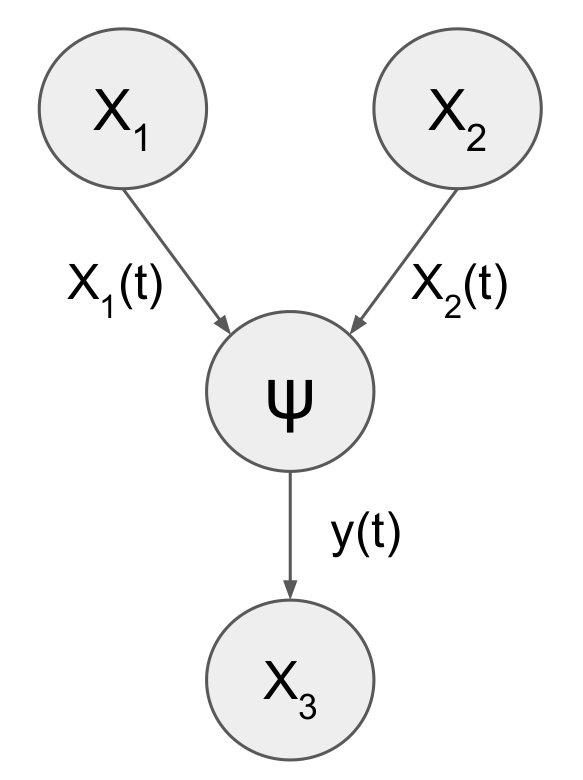
\includegraphics[width=3.5cm]{figures/simple_graph}
		\caption{Communication model.}
	\end{center}
	\label{fig:graph_model}
\end{wrapfigure} 
The communication model considered in this thesis is given in \autoref{fig:graph_model}. The parent nodes, $X_{1}$ and $ X_{2}$, emit messages which carry information about their states. These messages are translated by an observation model, $\psi$, and agent node, $ X_{3} $ makes a decision based on this translated message, $ y $. The main objective is to infer the observation model given set of trajectories of nodes.

The transition models of the nodes and the dependencies between them are modelled as continuous-time Bayesian network (CTBN), denoted by \textbf{X}. The network \textbf{X} represents a stohastic process over a structured multivariate state space $ \rchi = [\rchi_1,..., \rchi_n] $. 

The messages that are emitted by the parent nodes $X_{1}$ and $ X_{2} $ are modelled as independent homogeneous continuous-time Markov processes $X_{i}(t)$, with state space $ \rchi_{i} = \left\lbrace x_{1}, x_{2}, ..., x_{n} \right\rbrace  $ for $ i \in \left\lbrace 1,2 \right\rbrace $.

The agent node $ X_3 $ does not have a direct access to the messages, but observes a translation of them. The observation model is defined as the likelihood of a translation given the parent messages.
\begin{equation}
\psi \coloneqq p(y(t) \mid X_{1}(t), X_{2}(t))
\end{equation}
The agent  $ X_{3} $ is modelled as inhomogenouos continuous-time Markov process with state space $ \rchi_{3} = \left\lbrace x_{1}, x_{2}, ..., x_{n} \right\rbrace  $ and set of actions $ a \in \left\lbrace a_{0}, a_{1}, ..., a_{k}\right\rbrace  $ to choose from. 

Given the observation, the agent forms a belief over the parent states, $  b(x_{1}, x_{2}; t) $, that summarizes the past observations.\cite{KAELBLING199899} The policy of the agent, $ \pi(a \mid b) $, is assumed to be shaped by evolution (close) to optimality. Based on the belief state, the agent takes an action, which in the setting described above means to change its internal dynamics. 
\section{Continuous Time Bayesian Networks}
A continuous-time Bayesian network (CTBN) is a graphical model that represents a collection of nodes whose values evolve continuously over time. In CTBN framework, through a directed graph, the dependencies of a set of Markov processes (MPs) can be modelled efficiently relying on two assumptions. First assumption is that only one node can transition at a time. Secondly, the instantenous dynamics of each node depends only on its parent nodes. \cite{Cohn2010a, Nodelman1995} 
%In the following, every node of a CTBN is considered to be a Markov process.
\subsection{Continuous Time Markov Processes}
A continuous-time Markov process (CTMP) is a continuous-time stochastic process which satisfies Markov property, namely, the probability distribution over the states at a future time is conditionally independent of the past states given the current state.\cite{Cohn2010a} Let X be a CTMP with state space $ \rchi = \left\lbrace x_{1}, x_{2}, ..., x_{n} \right\rbrace  $. Then the Markov property can be written as follows:
\begin{equation}
	\operatorname{Pr}\left(X^{\left(t_{k}\right)}=x_{t_{k}} | X^{\left(t_{k-1}\right)}=x_{t_{k-1}}, \ldots, X^{\left(t_{0}\right)}=x_{t_{0}}\right)=\operatorname{Pr}\left(X^{\left(t_{k}\right)}=x_{t_{k}} | X^{\left(t_{k-1}\right)}=x_{t_{k-1}}\right)
\end{equation}
A CTMP is represented by its transition intensity matrix, $ \textbf{Q} $. In this matrix, the intensity $ q_{i} $ represents the instantaneous probability of leaving state $ x_{i} $ and $ q_{i,j} $ represents the instantaneous probability of switching from state $ x_{i} $ to $ x_{j} $. 
\begin{equation}
	\textbf{Q} = 
	\begin{bmatrix}
	-q_{1} & q_{1,2} & 	{\hdots}  & q_{1,n} \\
	q_{2,1} & -q_{2} & 	{\hdots}  & q_{2,n}  \\
	{\vdots}  & 	{\vdots}  & 	{\ddots}  & {\hdots}  \\
	q_{n,1} &  q_{n,2} &  {\hdots} & -q_{n}
	\end{bmatrix}
\label{eq:Q_matrix}
\end{equation}
where $ q_{i} = \sum_{i \neq j} q_{i,j}$.\cite{Nodelman1995}

\subsubsection{Homogenous Continuous Time Markov Processes}
A continuous-time Markov process is time-homogenous when the transition intensities do not depend on time. Let X be a homogenous CTMP, with transition intensity matrix $ \textbf{Q}_X $. Infinitesimal transition probability from state $ x_{i} $ to $ x_{j} $ in terms of the transition intensities $ q_{i,j} $ can be written as \cite{Cohn2010a}:
\begin{equation}
p_{i,j}(h)=\delta_{ij}+q_{i,j} h+o(h)
\label{eq:Markov_trans_func}
\end{equation}
where $ p_{i, j}(h) \equiv Pr(X(t+h)=x_j\mid X(t)=x_i) $ are Markov transition functions, $ \delta_{i,j} = \delta(x_i,x_j)$ is Kronecker delta and o(.) is a function decaying to zero faster than its argument.

The \textit{master equation} is then derived as follows:
\begin{align}
	p_{j}(t) &= \operatorname{Pr}(X(t) = x_{j}) \nonumber\\
		& =\sum_{\forall i} p_{i, j}(h) p_{i}(t-h) \nonumber \\
	\lim_{h\rightarrow 0} p_{j}(t) 
		& = \lim_{h\rightarrow 0} \sum_{\forall i} \left[ \delta_{ij}+q_{i,j} h+o(h)\right]  p_{i}(t-h) \nonumber \\ 
		& = \lim_{h\rightarrow 0} p_{j}(t-h) + \lim_{h\rightarrow 0} h \sum_{\forall i} q_{i,j} p_{i}(t-h) \nonumber \\
	\lim_{h\rightarrow 0} \frac{p_{j}(t) - p_{j}(t-h)}{h} 
		&= \lim_{h\rightarrow 0} \sum_{\forall i} q_{i,j} p_{i}(t-h) \nonumber\\
	\frac{d}{dt} p_{j}(t) & = \sum_{\forall i} q_{i,j} p_{i}(t)
%		& = \sum_{\forall i \neq j}\left[  q_{i,j} p_{i}(t) - q_{j,i} p_{j}(t) \right]\nonumber
	\label{eq:master_equation}
\end{align}
Equation \ref{eq:master_equation} can be written in matrix form:
\begin{equation}
\frac{d}{dt} p(t) = p(t)\textbf{Q}
\end{equation}
where the time-dependent probability distribution $ p(t) $ is a row vector with entries $ {p_{i}(t)}_{x_{i}\in \rchi} $. 
The solution of this ODE is, 
\begin{equation}
p(t)=p(0) \exp (t\textbf{Q})
\end{equation}
with initial distribution $ p(0) $.

The amount of time staying in a state $ x_{i} $ is exponentially distributed with parameter $ q_{i} $. The probability density function $ f $ and cumulative distribution function $ F $ for staying in the state $ x_{i} $ \cite{Nodelman1995}:
\begin{align}
f(t) & = q_{i} \exp \left(-q_{i} t\right), t\geq 0  \label{eq:f(t)_homo}\\
F(t) & = 1 - \exp \left(-q_{i} t\right), t\geq 0 
\end{align}
Given the transitioning from state $ x_{i} $, the probability of landing on state $ x_{j} $ is $ q_{i,j}/q_{i} $.
\paragraph*{Likelihood Function}
\label{sec:llh_of_homo}
Consider a single transition denoted as $ d = <x_{i},x_{j},t> $, where transition occurs from state $ x_{i} $ to $ x_{j} $ after spending t amount of time at state $ x_{i} $. The likelihood of this transition is the product of the probability of having remained at state $ x_{i} $ for that long, and the probability of transitioning to $ x_{j} $.
\begin{equation}
\operatorname{Pr}(d  \mid \textbf{Q}) = \left( q_{i}exp(-q_{i}t) \right) \left( \frac{q_{i,j}}{q_{i}} \right)
\end{equation}
The likelihood of a trajectory sampled from a homogenous CTMC, $ X^{[0,T]} $, can be decomposed as the product of the likelihood of single transitions. The sufficient statistics summarizing this trajectory can be written as $ T[x_{i}] $, total amount of time spent in state $ x_{i} $, $ M[x_{i}, x_{j}] $ total number of transitions from state $ x_{i} $ to $ x_{j} $. Then the likelihood of a trajectory $  X^{\left[0,T\right] } $ can be written as:
\begin{align}
\operatorname{Pr}(X^{[0,T]}  \mid \textbf{Q}) &=  \prod_{d \in X^{[0,T]}} \operatorname{Pr}(d \mid \textbf{Q}) \nonumber\\&=\left(\prod_{ i} q_{i}^{M[x_{i}]} \exp \left(-q_{i} T[x_{i}]\right)\right)\left(\prod_{ i} \prod_{ j \neq i} \left(\frac{q_{i,j}}{q_{i}}\right)^{M\left[x_{i}, x_{j}\right]}\right) \nonumber\\ & = \prod_{j \neq i}  exp(-q_{i,j}T[x_{i}])\ q_{i,j}^{M[x_{i},x_{j}]}
\label{eq:lh_traj_homo}
\end{align}
where $ M[x_{i}] = \sum_{j \neq i} M[x_{i}, x_{j}] $ is the total number transitions leaving state $ x_{i} $.


\subsubsection{Conditional Markov Processes}
A continuous-time Markov process is \textit{time-inhomogenous} when the transition intensities changes over time. In a CTBN, while every node is a Markov process, the leaf nodes are characterized as \textit{conditional} Markov processes, a type of inhomogeneous MP, where the intensities change over time, but not as a function of time rather as a function of parent states. \cite{Nodelman1995} 

Let X be a conditional Markov process, with a set of parents $ \textbf{U} = Par(X)$. Its intensity matrix, \textit{conditional intensity matrix}, $ \textbf{Q}_{X\given \textbf{U}} $ can be viewed as a set of homogenous intensity matrices $ \textbf{Q}_{X\given \textbf{u}} $, with entries $ q_{i,j \mid \textbf{u}} $ (similar to \autoref{eq:Q_matrix}), for each instantiation of parent nodes $ \textbf{U}(t) =\textbf{u} $.\cite{Nodelman1995} As a result, given a trajectory of parent nodes, X has a trajectory of intensity matrix as a combination of these homogenous matrices.
\begin{equation}
\textbf{Q}^{[0,T]} = [\textbf{Q}_{X\given \textbf{U}(t_0)}, \textbf{Q}_{X\given \textbf{U}(t_1)}, ..., \textbf{Q}_{X\given \textbf{U}(t_N)}],\ 0<t_0<t_1<...<t_N\leq T
\end{equation}

Markov transition function for a conditional Markov process can be written as follows:
\begin{align}
\operatorname{Pr}(X(t + h) = x_j \mid X(t)=x_i, \textbf{U}(t)=u, \textbf{Q}_{X\given \textbf{u}}) = \delta(i,j) + q_{i,j \mid \textbf{u}} h + o(h)
\label{eq:CIM_trans_funct}
\end{align}


\paragraph*{Likelihood Function}
Given the instantiation of its parents, the complete information on the dynamics of X is obtained. Then the likelihood of a trajectory drawn from a conditional MP $ X $ can be written similar to \autoref{eq:lh_traj_homo},
\begin{align}
\operatorname{Pr}(X^{[0,T]}  \mid \textbf{Q}_{X\given \textbf{U}}) &=  \left(\prod_{ \textbf{u}}\prod_{ i} q_{i\mid \textbf{u}}^{M[x_{i}\mid \textbf{u}]} \exp \left(-q_{i\mid \textbf{u}} T[x_{i}\mid \textbf{u}]\right)\right)\left(\prod_{ \textbf{u}}\prod_{ i} \prod_{ j \neq i} \left(\frac{q_{i,j\mid \textbf{u}}}{q_{i\mid \textbf{u}}}\right)^{M\left[x_{i}, x_{j}\mid \textbf{u}\right]}\right) \nonumber\\ & = \prod_{ \textbf{u}}\prod_{j\neq i}  exp(-q_{i,j\mid \textbf{u}}T[x_{i}\mid \textbf{u}]) \ q_{i,j\mid \textbf{u}}^{M[x_{i},x_{j}\mid \textbf{u}]}
\label{eq:lh_traj_cond}
\end{align}
with the sufficient statistics introduced in \autoref{sec:llh_of_homo} are also conditioned on parent nodes.
%Let X be an inhomogeneous Markov process. $  X^{\left[0,T\right] } $ is a trajectory sampled from this process with $ m $ number of transitions, $ 0 = t_{0} < t_{1} < ... < t_{m} $ are the times where transition occurred, and $ x_{t_{0}}, x_{t_{1}},..., x_{t_{m}} $ are the observed states. The likelihood of trajectory  $  X^{\left[0,T\right] } $ can be written as follows: 
%\begin{equation}
%\operatorname{Pr}(X^{[0,T]}  \mid \textbf{Q}) = \prod_{k=1}^{m} \left[ q_{x_{k-1}} (t_{k}) \exp \left(-\int_{t_{k-1}}^{t_{k}} q_{x_{k-1}}(u) d u\right) \frac{q_{x_{k-1}, x_{k}} (t_{k})}{q_{x_{k-1}}(t_{k})}\right] 
%\label{eq:lh_traj_inhomo}
%\end{equation}
%For inhomogeneous CTMP, Equation \ref{eq:f(t)_homo} becomes:
%\begin{equation}
%f(t) = q_{i}(t) \exp \left(-\int_{0}^{t} q_{i}(u) d u\right)
%\end{equation}
%Let X be an inhomogeneous Markov process. $  X^{\left[0,T\right] } $ is a trajectory sampled from this process with $ m $ number of transitions, $ 0 = t_{0} < t_{1} < ... < t_{m} $ are the times where transition occurred, and $ x_{t_{0}}, x_{t_{1}},..., x_{t_{m}} $ are the observed states. The likelihood of trajectory  $  X^{\left[0,T\right] } $ can be written as follows: 
%\begin{equation}
%\operatorname{Pr}(X^{[0,T]}  \mid \textbf{Q}) = \prod_{k=1}^{m} \left[ q_{x_{k-1}} (t_{k}) \exp \left(-\int_{t_{k-1}}^{t_{k}} q_{x_{k-1}}(u) d u\right) \frac{q_{x_{k-1}, x_{k}} (t_{k})}{q_{x_{k-1}}(t_{k})}\right] 
%\label{eq:lh_traj_inhomo}
%\end{equation}


\subsection{The CTBN Model}
Evidently, a homogenouos CTMP can be considered as a conditional MP whose set of parents is empty. Thus, a CTBN can be formed as a set of conditional Markov processes.

Let \textbf{X} be a CTBN with local variables $ X_n $, $ n \in \left\lbrace 1,...N \right\rbrace $, each with a state space $ \rchi_n $. Given the dependencies of each variable as set of its parents $ \textbf{U}_n = Par(X_n) $, the transition model of each local variable $ X_n $ is modelled as conditional Markov processes. \cite{Nodelman1995} In the following the set of all conditional transition intensity matrices are denoted as $ \textbf{\textit{Q}} $.

Consider a trajectory drawn from CTBN $ \textbf{X} $, such that $ \textbf{X}^{[0, T]} = \left\lbrace X_1^{[0,T]},  X_2^{[0,T]}, ...,  X_N^{[0,T]}\right\rbrace  $. Following \autoref{eq:lh_traj_cond}, the likelihood of this trajectory can be written as follows.
\begin{align}
\operatorname{Pr}( \textbf{X}  | \textbf{\textit{Q}} ) = \prod_{n=1}^{N} \prod_{\textbf{u} \in \mathcal{\textbf{U}}_{n}} \prod_{x_i \in \mathcal{X}_{n}} \prod_{x_j \in \mathcal{X}_{n} \backslash x_i}
\exp \left[q_{i,j\mid \textbf{u}}^{n} T_{n}[x_i\mid \textbf{u}]\right] (q_{i,j\mid \textbf{u}}^{n})^{M_{n}[x_i, x_j\mid \textbf{u}]}
\end{align}
where $ T_n[.] $ and $ M_n[.] $ indicates the sufficient statistics for $ X_n $

\section{Belief State in Partially Observable Markov Decision Processes}
\label{sec:belief_POMDP}
Partially observable Markov decision process (POMDP) framework provides a model of an agent which interacts with its environment, but unable to obtain certain information about its state. Instead, the agent gets an observation which is a stochastic function of the true state. The main goal, as similar to Markov decision processes (MDPs), is to learn a policy solving a task by optimizing a reward function. The problem of decision making under uncertainty can be decomposed into two parts for the agent. The first is \textit{state estimator} to keep a belief state which is a sufficient statistic of its past experiences, and the second is the \textit{optimal policy} which will give an action based on the belief state. \cite{Murphy2000,KAELBLING199899}

In the problem considered in this thesis, the agent node $ X_{3} $ cannot observe the incoming messages directly, rather a summary of them. This presents a POMDP problem. However, since the optimal policy of the agent is assumed to be given, the theory for policy optimization is skipped. In this section, update methods for belief state is introduced.

In the following, belief state refers to the posterior probability distribution over the environment states.

\subsection{Exact/Bayes(?) Belief State Update}
\label{sec:exact_update}
Consider a POMDP problem, with discrete state space \textit{S}, action space \textit{A}, observation space $ \Omega $. In a scneario where a compact representation of the \textit{transition model}, $ T(s, a, s^{\prime})$,  and \textit{observation model}, $ O(s^{\prime}, a, o) $, is available, the belief state update can be obtain via Bayes' theorem \cite{KAELBLING199899}:
\begin{align}
b^{\prime}\left(s^{\prime}\right) &=\operatorname{Pr}\left(s^{\prime} | o, a, b\right) \nonumber\\
&=\frac{\operatorname{Pr}\left(o | s^{\prime}, a, b\right) \operatorname{Pr}\left(s^{\prime} | a, b\right)}{\operatorname{Pr}(o | a, b)} \nonumber\\
&=\frac{\operatorname{Pr}\left(o | s^{\prime}, a\right) \sum_{s \in \mathcal{S}} \operatorname{Pr}\left(s^{\prime} | a, b, s\right) \operatorname{Pr}(s | a, b)}{\operatorname{Pr}(o | a, b)} \nonumber\\
&=\frac{O\left(s^{\prime}, a, o\right) \sum_{s \in \mathcal{S}} T\left(s,a, s^{\prime}\right) b(s)}{\operatorname{Pr}(o | a, b)}
\label{eq:discrete_belief_update}
\end{align}

\subsection{Filtering for CTMP}
\label{sec:filtering_CTMC}
Equation \ref{eq:discrete_belief_update} is discrete-time solution of belief state. However, since in the model described in Section 2.1, the parent nodes are modelled as CTMPs, thus the environment state for the agent is the state of a CTMP, the belief state should be solved in continuous-time. This is achieved by the inference of posterior probability of CTMP. \cite{article}

\textit{Filtering problem} in statistical context, as opposed to deterministic digital filtering, refers to inference of the conditional probability of the true state of the system at some point in time, given the history of observations. \cite{Godsill2019}

Let X be a CTMP with transition intensity matrix \textbf{Q}. Assume discrete-time observations denoted by $ y_{1}=y(t_{1}), ..., y_{N}=y(t_{N}) $. The belief state can be written as:
\begin{equation}
	b(x_{i};t_{N}) = \operatorname{Pr}(X(t_{N}) = x_{i} \mid y_{1}, ..., y_{N})
\end{equation}
From the master equation given in \autoref{eq:master_equation}, it follows that:
\begin{equation}
 \frac{d}{dt} b(x_{j};t)  = \sum_{\forall i} q_{i,j} b(x_{i};t)
\end{equation}
The time-dependent belief state $ b(t) $ is a row vector with $ \left\lbrace b(x_{i};t)_{x_{i} \in \rchi}\right\rbrace  $.
This posterior probability can be described by a system of ODEs:
%TODO ODE or system of ODEs
\begin{equation}
\frac{db(t)}{dt} = b(t)\textbf{Q}
\end{equation}
where the initial condition $ b(0) $ is row vector with $ \left\lbrace b(x_{i};t)_{x_{i} \in \rchi}\right\rbrace $ \cite{article}. The solution to this ODE is
\begin{equation}
b(t) = b(0) exp(t\textbf{Q}).
\label{eq:b_cont}
\end{equation}

The belief state update at discrete times of observation $ y_{t} $ is derived as 
\begin{align}
b(x_{i}; t_{N}) & = \operatorname{Pr}( X(t_{N}) = x_{i},\mid y_{1}, ..., y_{N}) \nonumber\\ & = \frac{\operatorname{Pr}(y_{1}, ..., y_{N}, X(t_{N}) = x_{i})}{\operatorname{Pr}(y_{1}, ..., y_{N})}  \nonumber\\ & = \frac{\operatorname{Pr}(y_{N} \mid y_{1}, ..., y_{N-1}, X(t_{N}) = x_{i})}{\operatorname{Pr}(y_{N} \mid y_{1}, ..., y_{N-1})} \frac{\operatorname{Pr}(y_{1}, ..., y_{N-1}, X(t_{N}) = x_{i})}{\operatorname{Pr}(y_{1}, ..., y_{N-1})}  \nonumber\\ & = Z_{N}^{-1} \ \operatorname{Pr}(y_{N} \mid X(t_{N})=x_{i})\ \operatorname{Pr}( X(t_{N}) = x_{i}\mid y_{1}, ..., y_{N-1})  \nonumber\\ & = Z_{N}^{-1}\ {\operatorname{Pr}(y_{N} \mid X(t_{N})=x_{i})}\ {b(x_{i}; t_{N}^{-})}
\label{eq:b_jump}
\end{align}
where $ Z_{N} = \sum_{x_{i}\in \rchi} \operatorname{Pr}(y_{N} \mid X(t_{N})=x_{i})\ b(x_{i}; t_{N}^{-}) $ is the normalization factor \cite{article}.

\subsection{Belief State Update using Particle Filter}
In a more realistic scenario, the exact update of belief state may not be feasible for several reasons. The computation of Bayes belief update is expensive for large state spaces. Moreover, a problem with continuous state spaces require a belief state represented as probability distributions over infinite state space rather than a collection of probabilities as given in Sec.\ref{sec:exact_update}. \cite{Carlo1904} Another reason could be lack of compact representation of transition and/or observation models. Under such circumstances, the belief state is obtained using sample-based approximation methods. \cite{Carlo1904} 

It should be noted that, since the belief state is nothing but the contidional probability of true states given the observations, the problem at hand poses a filtering problem as described in Section \ref{sec:filtering_CTMC}.

\subsubsection{Particle Filtering}
Particle filtering is one of the most commonly used Sequential Monte Carlo (SMC) algorithms. The popularity of this method thrives from the fact that, unlike other approximation methods such as Kalman Filter, it does not assume a linear Gaussion model. This advantage offers a great flexibility and finds application in a wide range of areas.\cite{Doucet2009}

The key idea in particle filtering is to approximate a target distribution $ p(x) $ by a set of samples (particles) drawn from that distribution. This is achieved sequentially updating the particles through two steps. First step is \textit{importance sampling}. Since the target distribution is not available, the particles are generated from a \textit{proposal distribution} $ q(x) $ and weighted in the account of the difference between target and proposal distributions. The second step is to resample the particles using these weights. \cite{Godsill2019}
%\begin{align*}
%	x^{(i)} & \sim q(x) \\
%	q(x) & \approx \frac{1}{N} \sum_{i=1}^{N} \delta_{x^{(i)}}(x) \\
%	w(x) & = \frac{p(x)}{q(x)}
%\end{align*}

In this application, the particles to represent the belief state are drawn from marginalized CTBN.
\subsubsection{Marginalized Continuous Time Markov Process}
Let \textbf{X} be a CTBN with local variables $ X_n $, $ n\in \left\lbrace 1,...,N \right\rbrace $, and set of conditional intensity matrices \textbf{\textit{Q}}. The marginal process description of \textbf{X} considering a single trajectory in interval $ [0,t) $ is given as follows:
\begin{multline}
\operatorname{Pr}(X_n(t + h) = x' \mid X_n(t)=x, U_n(t)=u, \textbf{X}^{[0, t)})\\
\begin{split}
&= \int \operatorname{Pr}(X_n(t + h) = x' \mid X_n(t)=x, U_n(t)=u, Q^u_n, \textbf{X}^{[0, t)})p(Q^u_n)dQ^u_n\\
&= \delta(x, x') + \mathbb{E}[Q^u_n (x, x') \mid \textbf{X}^{[0, t]} = \textbf{x}^{[0, t]}]h + o(h),
\end{split}
\end{multline}
By integrating out the intensity matrix $ Q^u_n $, the parameter is replaced by its expected value given the history of the process. It should be noted that by doing so, the process becomes parameter-free, and thus self-exciting. 

Consider K trajectories drawn from CTBN \textbf{X}, denoted by $ \xi_t = \left\lbrace \textbf{X}^{[0,t], 1}, \textbf{X}^{[0,t], 2}, ..., \textbf{X}^{[0,t], K} \right\rbrace  $. Since given Q

\begin{equation}
	p\left(Q | \mathbf{x}_{t}\right)=\frac{p\left(\mathbf{x}_{t} | Q\right) p(Q)}{p\left(\mathbf{x}_{t}\right)}
\end{equation}
\begin{align}
	p(\xi_{t} | Q ) = \prod_{n=1}^{N} \prod_{u \in \mathcal{U}_{n}} \prod_{x \in \mathcal{X}_{n}} \prod_{x^{\prime} \in \mathcal{X}_{n} \backslash x}
	\exp \left[Q_{n}^{u}\left(x, x^{\prime}\right) T_{n}^{u}(x)\right] Q_{n}^{u}\left(x, x^{\prime}\right)^{r_{n}^{u}\left(x, x^{\prime}\right)}
\end{align}
\begin{equation}
	\mathbb{E}\left[Q_{n}^{u}\left(x, x^{\prime}\right) | \xi_{t}\right]=\frac{\alpha_{n}^{u}\left(x, x^{\prime}\right)+r_{n}^{u}\left(x, x^{\prime}\right)}{\beta_{n}^{u}\left(x, x^{\prime}\right)+T_{n}^{u}(x)}
\end{equation}
%This expression also holds for $K$ trajectories that have been independently drawn from the CTBN; in line with the paper, we denote the joint history of all $K$ trajectories until time point $t$ as $\xi_t = \{x^1_{[0, t]}, ..., x^K_{[0, t]}\}$.
%
%By integrating out the rate matrices $Q^u_n$, we introduced dependencies between all trajectories; this is readily seen by evaluation of the above expectation:
%\begin{align}
%\mathbb{E}[Q^u_n (x, x') \mid \xi_t] &=\frac{\alpha^u_n(x, x') + r^u_n(x, x')}{\beta^u_n(x, x') + T^u_n(x)}\\
%&=\frac{\alpha^u_n(x, x') + \sum_k r^u_{n, k}(x, x')}{\beta^u_n(x, x') + \sum_k T^u_{n, k}(x)}.
%\end{align}
%The expectation of the rate matrix depends on the summary statistics $T^u_n = \sum_k T^u_{n,k}$, $r^u_n = \sum_k r^u_{n,k}$ from all observed trajectories up to the current point in time. Hence, to draw $K$ trajectories from a marginalised CTBN exactly, they have to be simulated jointly, inducing a joint path measure $p(\{X^k_{[0, T]} : k = 1, ..., K\})$.
%Because this is computationally infeasible, we would like to approximate this resulting joint distribution
%by a set of $K$ factorising variational distributions: $\prod_k q(X^k_{[0, T]})$ such that
%\begin{equation}
%\min_q \mathrm{KL}\,\left(\prod_k q(X^k_{[0, T]})\mid\mid p(\{X^k_{[0, T]}\}_k)\right).
%\end{equation}

	\externaldocument[-f]{c2_foundations}
\chapter{Experimental Setup}

This chapter presents the methodology used in this thesis. First, it is explained how different frameworks introduced in \autoref{chap:2} are put into use. Then, the algorithms used in data generation and inference is given in detail. The results from these experiments are presented in the succeeding chapter.

\section{The Model}
\begin{wrapfigure}{r}{3cm}
	\begin{center}
		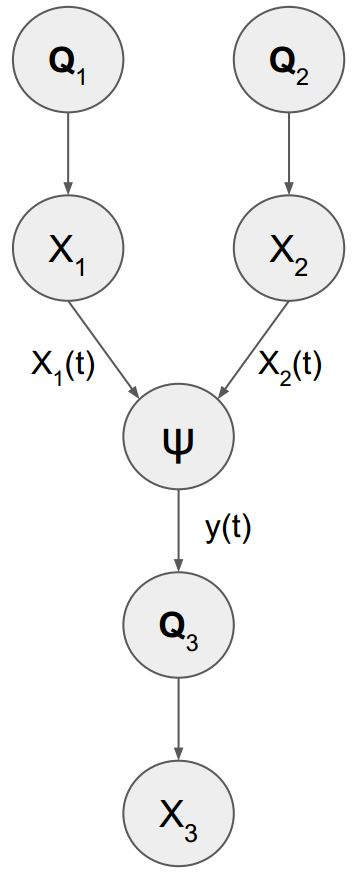
\includegraphics[width=2.5cm]{figures/h_model}
		\caption{Hierarchical model.}
	\end{center}
	\label{fig:h_model}
\end{wrapfigure} 
A detailed graphical model explored in this thesis is given in the \autoref{fig:h_model}. This model presents an intersection of continuous-time Bayesian network and partially observable Markov decision process frameworks. 
\begin{itemize}
	\item The transition models of the nodes $ X_1, X_2$ and $ X_3 $, and the dependencies between them are modelled as CTBN.
	\item The interaction of agent node $ X_3 $ and its environment is modelled as POMDP.
\end{itemize}

\subsection{CTBN Model}

The transition models of the nodes and the dependencies between them are modelled as continuous-time Bayesian network (CTBN), denoted by \textbf{X}. The network \textbf{X} represents a stohastic process over a structured multivariate state space $ \rchi = [\rchi_1, \rchi_2, \rchi_3] $. 

The parent nodes $X_{1}$ and $ X_{2} $ emits their states as messages. The dynamics  of these nodes are modelled as independent homogeneous continuous-time Markov processes $X_{i}(t)$, with binary-valued states $ \rchi_{i} = \left\lbrace 0, 1 \right\rbrace  $ for $ i \in \left\lbrace 1,2 \right\rbrace $. These processes are defined by transition intensity matrices $ \textbf{Q}_{i} $, which are in the following forms and assumed to be gamma distributed with shape and rate parameters $ \boldsymbol{\alpha} = [\alpha_0, \alpha_1] $ and $ \boldsymbol{\beta} = [\beta_0, \beta_1] $, respectively.
\begin{align}
\textbf{Q}_i &= 
\begin{bmatrix}
-q^i_{0} & q^i_{0} \\
q^i_{1} &  -q^i_{1}
\end{bmatrix}
\label{eq:Q_parents}\\
\textbf{Q}_{i} &\sim Gam(\boldsymbol{\alpha}^i, \boldsymbol{\beta}^i)\ \ for\ i \in \left\lbrace 1,2\right\rbrace \nonumber
\end{align}
It should be noted that in \autoref{eq:Q_parents}, the suffixes are simplified using the fact that $ q_{i} = \sum_{i \neq j} q_{i,j}$.

The agent  $ X_{3} $ is modelled as inhomogenouos continuous-time Markov process with binary states $ \rchi_{3} = \left\lbrace 0, 1 \right\rbrace  $ and set of actions $ a \in \left\lbrace a_0, a_1\right\rbrace  $, and set of transition intensity matrices which contains one matrix corresponding to each action, $ \textbf{\textit{Q}}_{3} = \left\lbrace \textbf{Q}_{a_{0}}, \textbf{Q}_{a_{1}} \right\rbrace $.
%\begin{equation}
%\textbf{Q}_{a_k} \sim Gam(\alpha_{a_k}, \beta_{a_k})
%\end{equation}

The dependencies are represented by set of parents for each node $ \textbf{U}_{X_{n}} = Par(X_n) $ and for the model shown in \autoref{fig:h_model} can be written as follows:
\begin{align*}
\textbf{U}_{X_{1}}, \textbf{U}_{X_{2}} & = \emptyset \\
\textbf{U}_{X_{3}} & = \left\lbrace X_1, X_2 \right\rbrace 
\end{align*}

\subsection{POMDP Model}
In a conventional POMDP scenario, there are two problem to be addressed, one is belief state update and the other is policy optimization. As mentioned in \autoref{sec:belief_POMDP}, in the problem at hand, the policy of agent $ X_3 $ is assumed to be optimal and given. Thus, the POMDP model of the agent only consists of belief state update. A detailed view of the agents interaction from POMDP framework perspective is given in the \autoref{fig:POMDP_pers}. \\
\textbf{SHOULD I ADD 'inspired by ...' WITH CITATION TO POMDP PAPER?}\\
\begin{figure}[htb]
	\begin{center}
		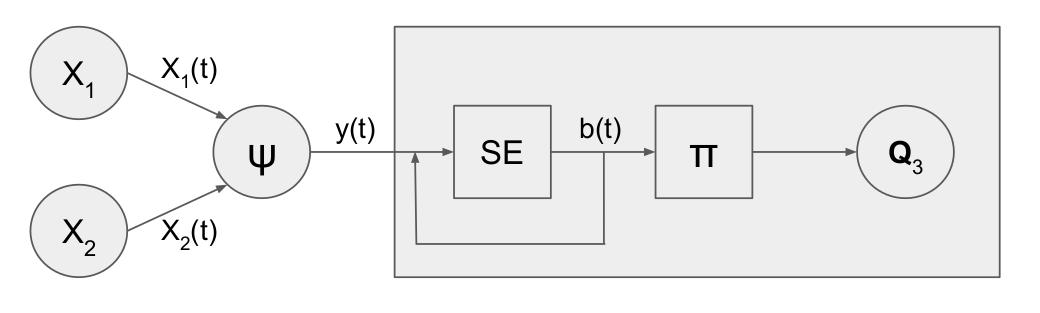
\includegraphics[width=.75\textwidth]{figures/POMDP_pers}
		\caption{Closer look to agent-environment interaction from the perspective of POMDP framework.}
		\label{fig:POMDP_pers}
	\end{center}
\end{figure}\\
The agent node $ X_3 $ does not have a direct access to the messages, but observes a translation of them. The observation model is defined as the likelihood of a translation given the parent messages.
\begin{equation}
\psi \coloneqq \operatorname{Pr}(y(t) \mid X_{1}(t), X_{2}(t))
\end{equation}
The state estimator (labelled as SE in \autoref{fig:POMDP_pers}) forms a belief over the parent states, $  b(x_{1}, x_{2}; t) $. 
\begin{equation}
b(x_{1}, x_{2}; t) = \operatorname{Pr}( X_{1}(t) = x_{1},  X_{2}(t) = x_{2}\mid y_{1}, ..., y_{t})
\end{equation}
Given the optimal policy, $ \pi(b(t)) $, the agent takes an action based on the belief state. In the setting described above, taking an action means to change its internal dynamics to the transition intensity matrix corresponding to that action.
\begin{align}
a(t) &= \pi(b(t))\\
\textbf{Q}_3(t) & = \textbf{\textit{Q}}_3[a(t)]
\end{align}
\textbf{WORK ON THESE NOTATIONS}\\

\subsubsection{POMDP Model with Exact Belief State Update}
Given the transition intensity matrices of parent nodes, $ \textbf{Q}_1 $ and $ \textbf{Q}_2 $, the belief state update poses a filtering problem for CTMPs (\autoref{sec:filtering_CTMC}). 

Consider a subsystem of CTBN model, consisting of only the parent nodes, $ X_1 $ and $ X_2 $. These two processes can be represented as one single \textit{joint} process, P, with joint state space $ \textit{P} = \left\lbrace (x_1, x_2)\right\rbrace  = \left\lbrace (0,0), (0,1), (1,0), (1,1)\right\rbrace  $. The transition intensity matrix of the new joint system, $ \textbf{Q}_P $ is obtained by amalgamation operation between $ \textbf{Q}_{1} $ and  $ \textbf{Q}_{2} $ \cite{Nodelman1995}.
%TODO x_1 and x_2 notation is not mentioned before, clarify!
\begin{equation}
\textbf{Q}_P = \textbf{Q}_{1} * \textbf{Q}_{2}
\end{equation}
\textbf{AMALGAMATION EXPLANATION AT APPENDIX?}\\
Consider discrete-time observations, denoted by $ y_{1}=y(t_{1}), ..., y_{N}=y(t_{N}) $. Following \autoref{eq:b_cont} and \autoref{eq:b_jump}, the belief state update is evaluated as
%TODO give initial condition
\begin{equation}
b(t) = b(0) \exp(t\textbf{Q}_P)
\end{equation}
with reset condition at discrete times of observation $ y_{t} $ 
\begin{align}
b(x_{i}; t_{N}) &= Z_{N}^{-1}\ {\operatorname{Pr}(y_{N} \mid X(t_{N})=x_{i})}\ {b(x_{i}; t_{N}^{-})} \\ & = Z_{N}^{-1}\ \psi \ {b(x_{i}; t_{N}^{-})}
\end{align}
where $ Z_{N} = \sum_{x_{i}\in \rchi} \operatorname{Pr}(y_{N} \mid X(t_{N})=x_{i})\ b(x_{i}; t_{N}^{-}) $ is the normalization factor.

\subsubsection{POMDP Model with Belief State Update Using Particle Filter}

\scalebox{1}{\begin{algorithm}[H]
		\KwIn{Measurement data $ y_{k} $ at time $ t_{k} $, set of particles $\textbf{p}^{k-1} $, estimated $ \hat{Q} $}
		\KwResult{New set of particles $ \textbf{p}^{k} $, representing $ b(t_{k}) $}
		\vspace{+4pt}
		\begin{algorithmic}[1]
			\FOR{$p_{m} \in \textbf{p}^{k-1}$}
			\STATE {$p_{m} = \left\lbrace x_{m}, \hat{Q}\right\rbrace \leftarrow Propagate\ particle\ through\ marginal\ process\ model\ from\ t_{k-1}\ to\ t_{k}$ }
			\STATE{$w_{m} \leftarrow p(y_{k} \mid X(t_{k})=x_{m}) $} 
			\tcp*[h] {observation likelihood}
			\STATE {$\hat{Q} \leftarrow sufficient\ statistics\ added\ from\  p_{m}[t_{k-1}, t_{k}]$}
			\ENDFOR
			\STATE{$ w_{m} \leftarrow \frac{w_{m}}{\sum_{m} w_{m}}$} \tcp*[h]{normalize weights}
			\FOR{$ p_{m} \in \textbf{p}_{k} $} 
			\STATE{$ p_{m} \leftarrow Sample\ from\ p_{k}\ with\ probabilities\ w_{m}\ with\ replacement$}
			\ENDFOR
		\end{algorithmic}
		\caption{Marginal particle filter}
\end{algorithm}}
\subsubsection{Optimal Policy}

The optimal policy is defined as a polynomial function of belief state.
\begin{align}
\pi(b(t)) = \textbf{w}\ b(t)^T
\end{align}
where \textbf{w} is a row vector of weights.\\
\textbf{INCONSISTENT WITH NOTATION USED BEFORE}

\section{Data Generation}
\subsection{Sampling Trajectories}
\subsubsection{Gillespie Algorithm}
\subsubsection{Thinning Algorithm}
\section{Inference of Observation Model}
Our dataset contains a number of trajectories from all the nodes involved in the communication. $ \textbf{D} = \left\lbrace D_{1},..., D_{N}\right\rbrace $. Every trajectory comprises of state transitions in time interval $  [0, T] $, and the times of these transitions.


\section{Parameters}

\paragraph{Marginalized Likelihood Function} 
Let $ X $ be a homogenous CTMP. For convenience, it is assumed to be binary-valued, $ \rchi = \left\lbrace x_{0}, x_{1} \right\rbrace $. The transition intensity matrix can be written in the following form:
\begin{equation}
\textbf{Q} = 
\begin{bmatrix}
-q_{0} & q_{0} \\
q_{1} & -q_{1}
\end{bmatrix}
\end{equation}
where the transition intensities $ q_{0} $ and $ q_{1} $ are gamma-distributed with parameters $ \alpha_{0}$, $ \beta_{0} $ and $ \alpha_{1} $, $ \beta_{1} $, respectively. The marginal likelihood of a sample trajectory $ X^{[0,T]} $ can be written as follows:
\begin{align}
P(X^{[0, T]}) & = \int  P(X^{[0, T]}\mid Q)P(Q) dQ \nonumber\\ & = \int_{0}^{\infty} \left( \prod_{x} \exp(-q_{x}T_{x}) \prod_{x'} q_{xx'}^{M[x, x']}\right) \frac{\beta_{xx'}^{\alpha_{xx'}}{q_{xx'}^{\alpha_{xx'}-1}}\exp(-\beta_{xx'}q_{xx'})}{\Gamma(\alpha_{xx'})} \ dq_{xx'} \nonumber\\ & = \prod_{i\in{0,1}}\int_{0}^{\infty} q_{i}^{M[x_{i}]} \ \exp(-q_{i}T[x_{i}]) \  \frac{\beta_{i}^{\alpha_{i}} \ q_{i}^{\alpha_{i}-1}\ \exp(-\beta_{i}q_{i})}{\Gamma(\alpha_{i})} \ dq_{i} \nonumber\\ & = \prod_{i\in{0,1}} \frac{\beta_{i}^{\alpha_{i}}}{\Gamma(\alpha_{i})} \int_{0}^{\infty} q_{i}^{M[x_{i}] + \alpha_{i} -1} \ \exp(-q_{i}(T[x_{i}]+\beta_{i})) \ dq_{i} \\ & = \prod_{i\in{0,1}} \frac{\beta_{i}^{\alpha_{i}}}{\Gamma(\alpha_{i})} \left( -(T_{i}+\beta_{i})^{M[x_{i}] + \alpha_{i}}\ \Gamma(M[x_{i}] + \alpha_{i}, \ q_{i}(T[x_{i}]+\beta_{i})) \right) \Big|_0^\infty  \\ & = \prod_{i\in{0,1}} \frac{\beta_{i}^{\alpha_{i}}}{\Gamma(\alpha_{i})} \left( (T[x_{i}]+\beta_{i})^{M[x_{i}] + \alpha_{i}}\ \Gamma(M[x_{i}] + \alpha_{i}) \right)
\label{eq:Marg_traj}
\end{align}.
%
%where $ T[x_{i}] $, the amount of time spent in state $ [x_{i}] $, $ M[x_{i},x_{j}] $ the number of transitions from state $ x_{i} $ to $ x_{j} $ and  $ M[x_{i}] = \sum_{i\neq j}M[x_{i},x_{j}] $.\\

%From Eq.11, the integral is solved using computer algebra system WolframAlpha as follows:
%\begin{align}
%\int x^{a} \ \exp(-xb) \ dx = -b^{-a-1} \ \Gamma(a+1, \ bx) + C
%\label{eq:integral}
%\end{align}
%
%Plugging Eq.\ref{eq:Marg_traj} in Eq.\ref{eq:Marg_llh} for both $ X_{1} $ and $ X_{2} $:
%\begin{align}
%\begin{split}
%P(\textit{D} \mid \pi, \Phi ) = P(X_{3}^{[0, T]}\mid Q_{3}^{[0, T]}) \prod_{x_{1}\in{0,1}} \frac{\beta_{x_{1}}^{\alpha_{x_{1}}}}{\Gamma(\alpha_{x_{1}})} \ (T_{x_{1}}+\beta_{x_{1}})^{M_{x_{1}} + \alpha_{x_{1}}}\ \Gamma(M_{x_{1}} + \alpha_{x_{1}})  \\  \prod_{x_{2}\in{0,1}} \frac{\beta_{x_{2}}^{\alpha_{x_{2}}}}{\Gamma(\alpha_{x_{2}})} \ (T_{x_{2}}+\beta_{x_{2}})^{M_{x_{2}} + \alpha_{x_{2}}}\ \Gamma(M_{x_{2}} + \alpha_{x_{2}})
%\label{eq:Marg_llh_final}
%\end{split}
%\end{align}

	\chapter{Results}


\section{Simulation}
\begin{figure}[htb]
	\begin{center}
		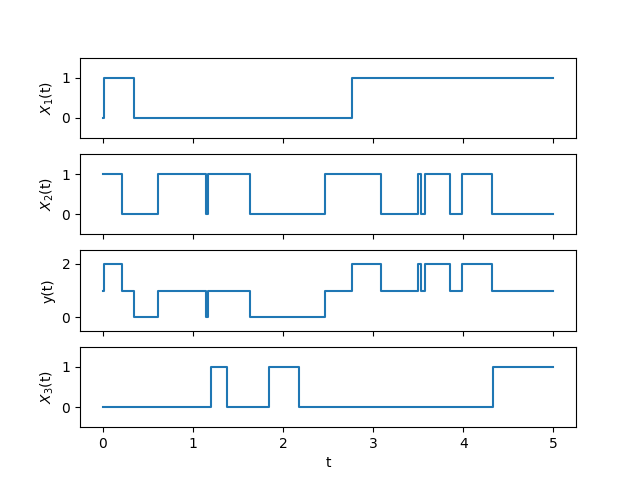
\includegraphics[width=.50\textwidth]{figures/traj}
		\caption{Sampled trajectories}
		\label{fig:traj}
	\end{center}
\end{figure}
\begin{figure}[htb]
	\begin{center}
		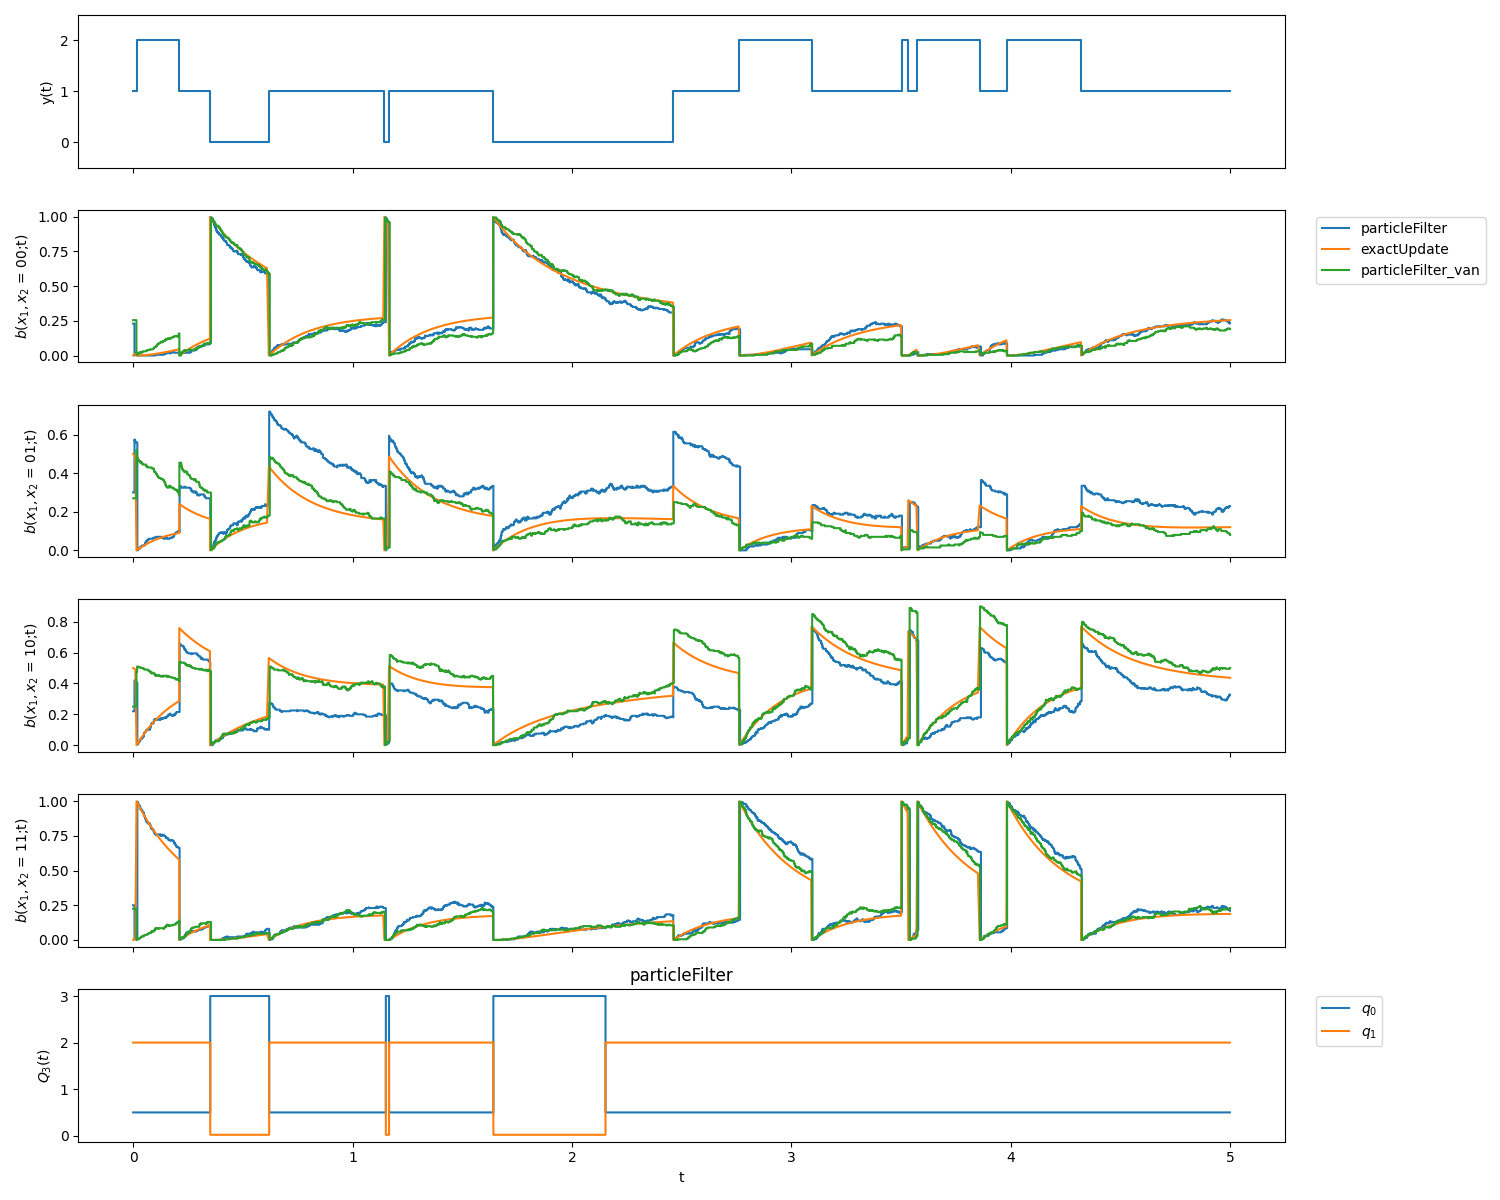
\includegraphics[width=.50\textwidth]{figures/b_q_traj}
		\caption{Belief state and $ Q_3 $ trajectories}
		\label{fig:b_q_traj}
	\end{center}
\end{figure}

\section{Results}
\subsection{Maximum Likelihood Estimation}
$\psi_{true} =
\begin{bmatrix} \vspace{-2pt}
	1 & 0 & 0 \\  \vspace{-2pt}
	0 & 1 & 0 \\  \vspace{-2pt}
	0 & 1 & 0 \\  \vspace{-1pt}
	0 & 0 & 1
\end{bmatrix}$
$\psi_{0} =
\begin{bmatrix} \vspace{-2pt}
1 & 0 & 0 \\  \vspace{-2pt}
0 & 1 & 0 \\  \vspace{-2pt}
0 & 1 & 0 \\  \vspace{-1pt}
0 & 0 & 1
\end{bmatrix}, 
\psi_{1} =
\begin{bmatrix} \vspace{-2pt}
0 & 0 & 1 \\  \vspace{-2pt}
0 & 1 & 0 \\  \vspace{-2pt}
1 & 0 & 0 \\  \vspace{-1pt}
0 & 0 & 1 
\end{bmatrix},
\psi_{2} =
\begin{bmatrix} \vspace{-2pt}
0 & 0 & 1 \\  \vspace{-2pt}
1 & 0 & 0 \\  \vspace{-2pt}
0 & 0 & 1 \\  \vspace{-1pt}
0 & 1 & 0  
\end{bmatrix}$
\begin{figure}[htb]
	\begin{subfigure}{.5\textwidth}
		\centering
		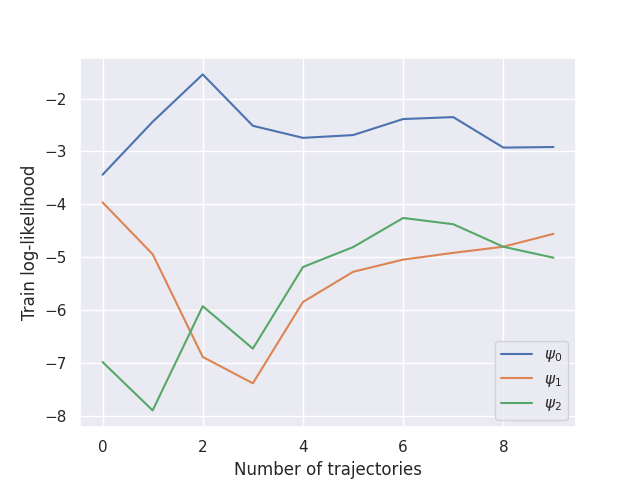
\includegraphics[width=1\linewidth]{figures/llh_[1.0, 0.0, 0.0]}
		\caption{}
		\label{fig:sfig1}
	\end{subfigure}%
	\begin{subfigure}{.5\textwidth}
		\centering
		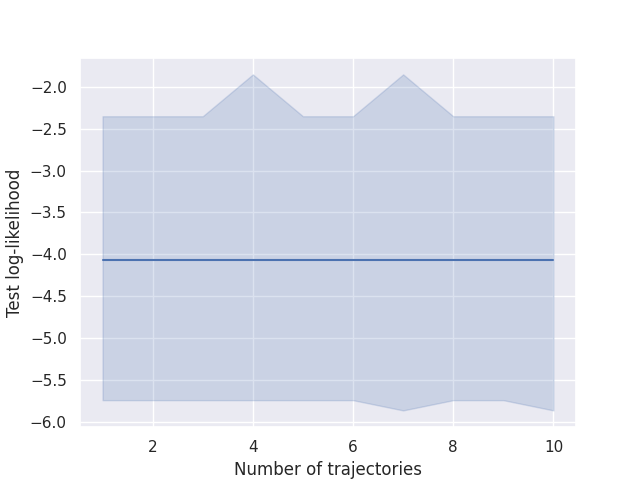
\includegraphics[width=1\linewidth]{figures/test_likelihood_particleFilter_[1.0, 0.0, 0.0]}
		\caption{}
		\label{fig:sfig2}
	\end{subfigure}
	\caption{plots of....}
	\label{fig:fig}
\end{figure}\\
$\psi_{true} =
\begin{bmatrix} \vspace{-2pt}
0.98 & 0.01 & 0.01 \\  \vspace{-2pt}
0.01 & 0.98 & 0.01 \\  \vspace{-2pt}
0.01 & 0.98 & 0.01 \\  \vspace{-1pt}
0.01 & 0.01 & 0.98
\end{bmatrix}$
$\psi_{0} =
\begin{bmatrix} \vspace{-2pt}
1 & 0 & 0 \\  \vspace{-2pt}
0 & 1 & 0 \\  \vspace{-2pt}
0 & 1 & 0 \\  \vspace{-1pt}
0 & 0 & 1
\end{bmatrix}, 
\psi_{1} =
\begin{bmatrix} \vspace{-2pt}
0 & 0 & 1 \\  \vspace{-2pt}
0 & 1 & 0 \\  \vspace{-2pt}
1 & 0 & 0 \\  \vspace{-1pt}
0 & 0 & 1 
\end{bmatrix},
\psi_{2} =
\begin{bmatrix} \vspace{-2pt}
0 & 0 & 1 \\  \vspace{-2pt}
1 & 0 & 0 \\  \vspace{-2pt}
0 & 0 & 1 \\  \vspace{-1pt}
0 & 1 & 0  
\end{bmatrix}$
\begin{figure}[htb]
	\begin{subfigure}{.5\textwidth}
		\centering
		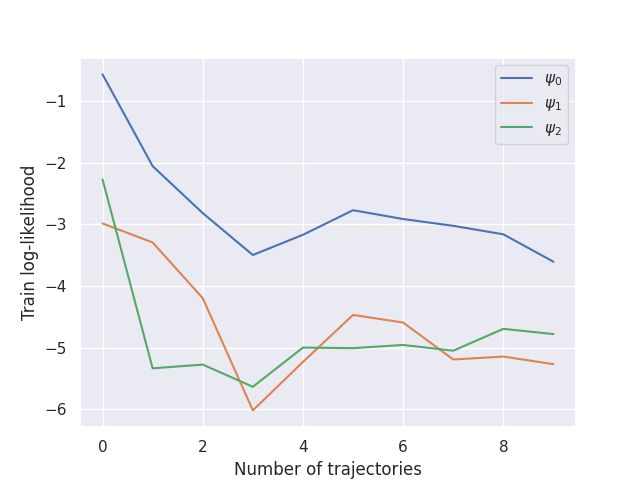
\includegraphics[width=1\linewidth]{figures/llh_[0.98, 0.01, 0.01]}
		\caption{}
		\label{fig:sfig1}
	\end{subfigure}%
	\begin{subfigure}{.5\textwidth}
		\centering
		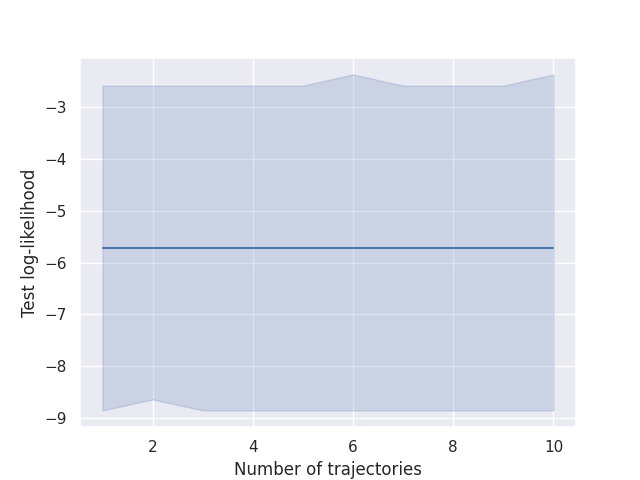
\includegraphics[width=1\linewidth]{figures/test_likelihood_particleFilter_[0.98, 0.01, 0.01]}
		\caption{}
		\label{fig:sfig2}
	\end{subfigure}
	\caption{plots of....}
	\label{fig:fig}
\end{figure}\\
$\psi_{true} =
\begin{bmatrix} \vspace{-2pt}
0.95 & 0.025 & 0.025 \\  \vspace{-2pt}
0.025 & 0.95 & 0.025 \\  \vspace{-2pt}
0.025 & 0.95 & 0.025 \\  \vspace{-1pt}
0.025 & 0.025 & 0.95
\end{bmatrix}$
$\psi_{0} =
\begin{bmatrix} \vspace{-2pt}
1 & 0 & 0 \\  \vspace{-2pt}
0 & 1 & 0 \\  \vspace{-2pt}
0 & 1 & 0 \\  \vspace{-1pt}
0 & 0 & 1
\end{bmatrix}, 
\psi_{1} =
\begin{bmatrix} \vspace{-2pt}
0 & 0 & 1 \\  \vspace{-2pt}
0 & 1 & 0 \\  \vspace{-2pt}
1 & 0 & 0 \\  \vspace{-1pt}
0 & 0 & 1 
\end{bmatrix},
\psi_{2} =
\begin{bmatrix} \vspace{-2pt}
0 & 0 & 1 \\  \vspace{-2pt}
1 & 0 & 0 \\  \vspace{-2pt}
0 & 0 & 1 \\  \vspace{-1pt}
0 & 1 & 0  
\end{bmatrix}$
\begin{figure}[htb]
	\begin{subfigure}{.5\textwidth}
		\centering
		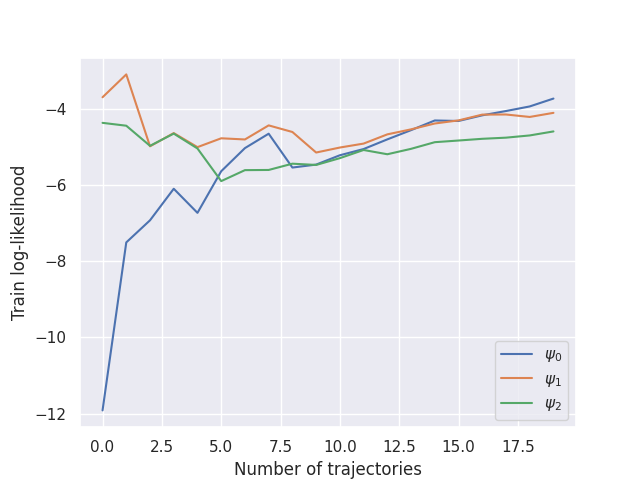
\includegraphics[width=1\linewidth]{figures/llh_particleFilter_[0.95, 0.025, 0.025]}
		\caption{}
		\label{fig:sfig1}
	\end{subfigure}%
	\begin{subfigure}{.5\textwidth}
		\centering
		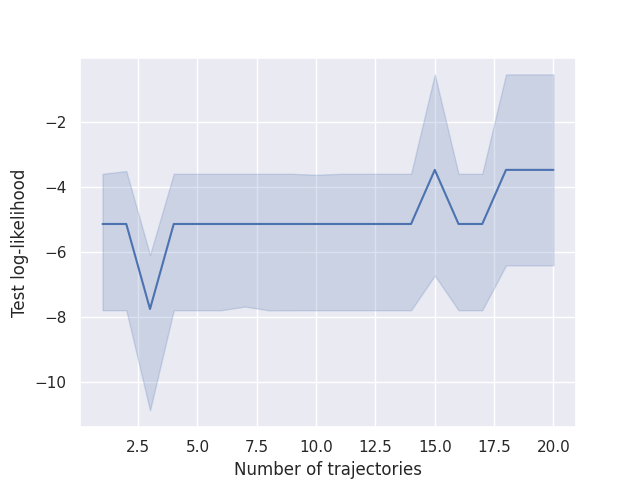
\includegraphics[width=1\linewidth]{figures/test_likelihood_particleFilter_[0.95, 0.025, 0.025]}
		\caption{}
		\label{fig:sfig2}
	\end{subfigure}
	\caption{plots of....}
	\label{fig:fig}
\end{figure}\\
$\psi_{true} =
\begin{bmatrix} \vspace{-2pt}
0.9 & 0.05 & 0.05 \\  \vspace{-2pt}
0.05 & 0.9 & 0.05 \\  \vspace{-2pt}
0.05 & 0.9 & 0.05 \\  \vspace{-1pt}
0.05 & 0.05 & 0.9
\end{bmatrix}$
$\psi_{0} =
\begin{bmatrix} \vspace{-2pt}
1 & 0 & 0 \\  \vspace{-2pt}
0 & 1 & 0 \\  \vspace{-2pt}
0 & 1 & 0 \\  \vspace{-1pt}
0 & 0 & 1
\end{bmatrix}, 
\psi_{1} =
\begin{bmatrix} \vspace{-2pt}
0 & 0 & 1 \\  \vspace{-2pt}
0 & 1 & 0 \\  \vspace{-2pt}
1 & 0 & 0 \\  \vspace{-1pt}
0 & 0 & 1 
\end{bmatrix},
\psi_{2} =
\begin{bmatrix} \vspace{-2pt}
0 & 0 & 1 \\  \vspace{-2pt}
1 & 0 & 0 \\  \vspace{-2pt}
0 & 0 & 1 \\  \vspace{-1pt}
0 & 1 & 0  
\end{bmatrix}$
\begin{figure}[htb]
	\begin{subfigure}{.5\textwidth}
		\centering
		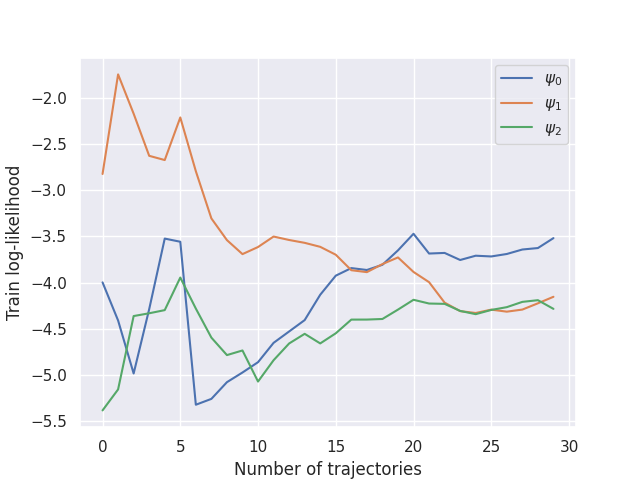
\includegraphics[width=1\linewidth]{figures/llh_particleFilter_van}
		\caption{}
		\label{fig:sfig1}
	\end{subfigure}%
	\begin{subfigure}{.5\textwidth}
		\centering
		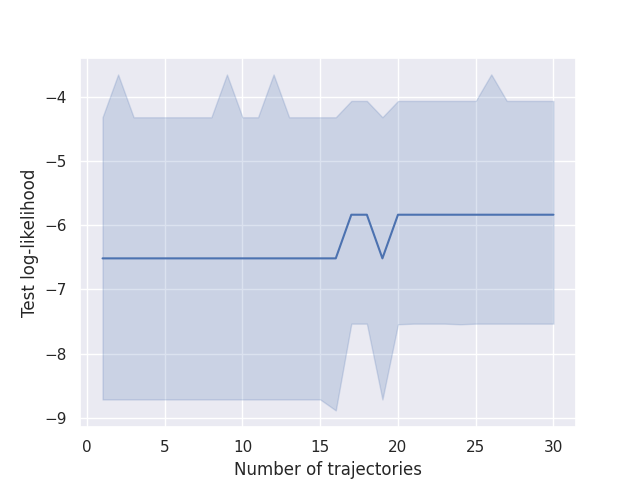
\includegraphics[width=1\linewidth]{figures/test_likelihood_particleFilter_van}
		\caption{}
		\label{fig:sfig2}
	\end{subfigure}
	\caption{plots of....}
	\label{fig:fig}
\end{figure}

\subsection{Maximum Likelihood Classification}
\begin{figure}[htb]
	\begin{subfigure}{.33\textwidth}
		\centering
		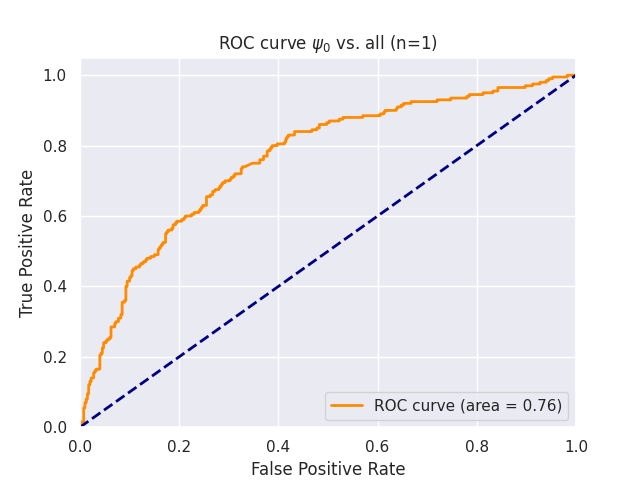
\includegraphics[width=1\linewidth]{figures/AUROC_600samples_class0_llh_n1}
		\caption{}
		\label{fig:sfig1}
	\end{subfigure}%
	\begin{subfigure}{.33\textwidth}
		\centering
		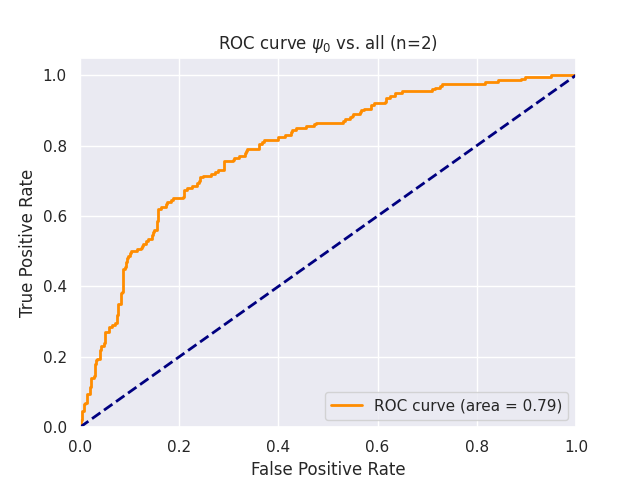
\includegraphics[width=1\linewidth]{figures/AUROC_600samples_class0_llh_n2}
		\caption{}
		\label{fig:sfig2}
	\end{subfigure}
	\begin{subfigure}{.33\textwidth}
		\centering
		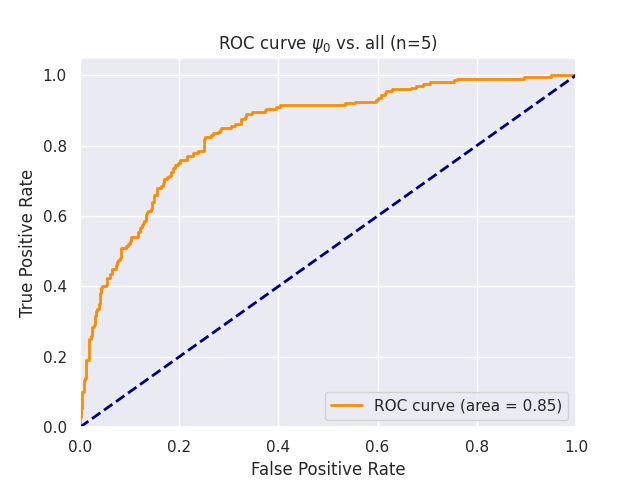
\includegraphics[width=1\linewidth]{figures/AUROC_600samples_class0_llh_n5}
		\caption{}
		\label{fig:sfig2}
	\end{subfigure}\\
	\begin{subfigure}{.33\textwidth}
		\centering
		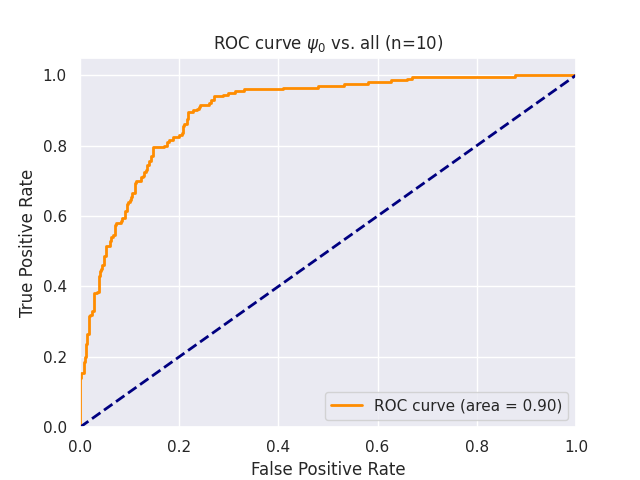
\includegraphics[width=1\linewidth]{figures/AUROC_600samples_class0_llh_n10}
		\caption{}
		\label{fig:sfig1}
	\end{subfigure}%
	\begin{subfigure}{.33\textwidth}
		\centering
		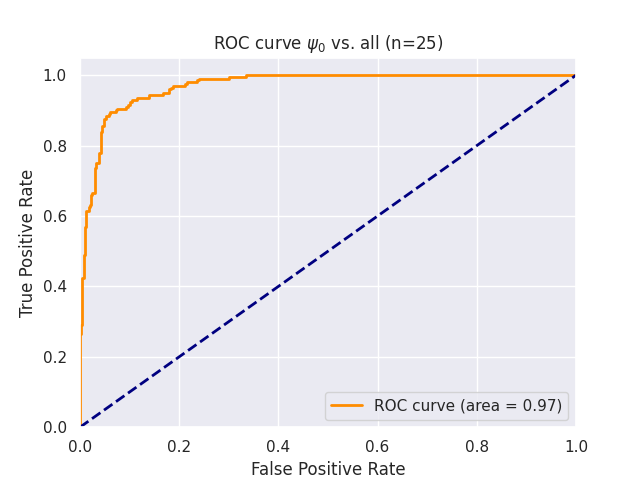
\includegraphics[width=1\linewidth]{figures/AUROC_600samples_class0_llh_n25}
		\caption{}
		\label{fig:sfig2}
	\end{subfigure}
	\begin{subfigure}{.33\textwidth}
		\centering
		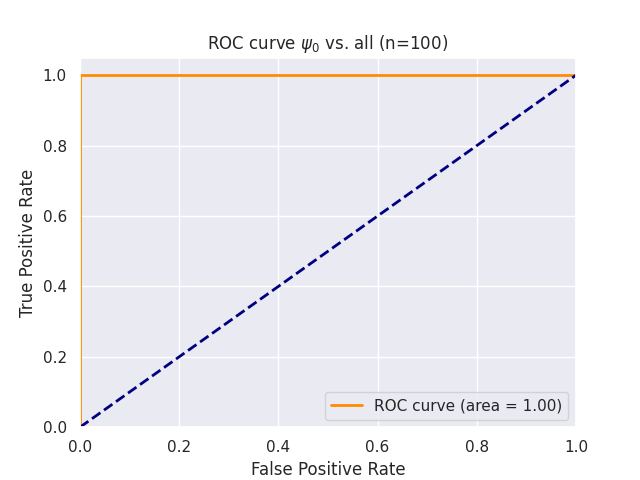
\includegraphics[width=1\linewidth]{figures/AUROC_600samples_class0_llh_n100}
		\caption{}
		\label{fig:sfig2}
	\end{subfigure}\\
	\caption{plots of....}
	\label{fig:fig}
\end{figure}
\begin{figure}[htb]
	\begin{center}
		\includegraphics[width=.9\textwidth]{figures/all_particlefilter}
		\caption{plot of...}
		\label{fig:traj}
	\end{center}
\end{figure}

	\chapter{Conclusion}
\blindtext

\section{Discussion}
\Blindtext
\Blindtext

\section{Future Work}
\Blindtext
	\bibliography{../bibtex/master_thesis}
\end{document}